


\begin{table}[t]
\begin{minipage}[b]{0.49\linewidth}
\centering

\small
    \addtolength{\tabcolsep}{-2pt}    
\caption{Open-Domain QA Test Scores. For TQA,  left column uses the standard test set for  Open- Domain QA, right column uses the TQA-Wiki test set. See Appendix \ref{sec:qa_appendix} for further details.}
\vspace{5pt}
    \resizebox{\textwidth}{!}{

    \begin{tabular}{llcc@{/}ccc}
    \toprule
          \multicolumn{2}{c}{Model} & NQ & \multicolumn{2}{c}{TQA} & WQ & CT \\\midrule
         \multirow{2}{0.12\linewidth}{Closed Book}&T5-11B \cite{roberts2020t5cqba} & 34.5 &- & 50.1 & 37.4& -\\
         &\scriptsize{T5-11B+SSM\cite{roberts2020t5cqba}}& 36.6 & - & 60.5 & 44.7 & - \\
         \midrule
         \multirow{2}{0.12\linewidth}{Open Book} &REALM \cite{guu2020realm} & 40.4 & - & - & 40.7 & 46.8 \\
         & DPR \cite{Karpukhin20dense} & 41.5 & \textbf{57.9} & - & 41.1 & 50.6 \\
         \midrule
         &{\ragtoken{}} & 44.1 &	55.2 & 66.1	& \textbf{45.5} & 50.0 \\
         &{RAG-Seq.} &  \textbf{44.5}&	56.8& \textbf{68.0} &	45.2&	\textbf{52.2} \\
    \bottomrule
    \end{tabular}
    }
    \addtolength{\tabcolsep}{2pt}    


    \label{tab:qa_results_table}
\end{minipage}
\hspace{0.01\linewidth}
\begin{minipage}[b]{0.49\linewidth}
\centering
  \caption{Generation and classification Test Scores.  MS-MARCO SotA is \cite{Bi2020PALMPA}, FEVER-3 is \cite{Zhong2019ReasoningOS} and FEVER-2 is \cite{Thorne2020AvoidingCF} *Uses gold context/evidence. Best model without gold access underlined. 
    }
    \vspace{13pt}
 \small
    \addtolength{\tabcolsep}{-3pt}   
\resizebox{\textwidth}{!}{
    \begin{tabular}{lccccccc}
    \toprule
          \multicolumn{1}{c}{Model}  & \multicolumn{2}{c}{Jeopardy} & \multicolumn{2}{c}{MSMARCO} & FVR3 & FVR2 \\
          \multicolumn{1}{c}{}& \multicolumn{1}{c}{B-1} & \multicolumn{1}{c}{QB-1} &\multicolumn{1}{c}{R-L} & \multicolumn{1}{c}{B-1} & \multicolumn{2}{c}{Label Acc.} \\\midrule
         SotA & - &	- &	\textbf{49.8}* & \textbf{49.9}*	 & \textbf{76.8} & \textbf{92.2}* \\\midrule
         BART & 15.1 &	19.7 &	38.2&	41.6 & 64.0 & 81.1 \\\midrule
        RAG-Tok. & \textbf{17.3}&	\textbf{22.2}&	40.1 &  41.5 & \multirow{2}{*}{72.5} & \multirow{2}{*}{\underline{89.5}} \\
         RAG-Seq. & 14.7	&21.4&	\underline{40.8} & \underline{44.2}\\
    \bottomrule
    \end{tabular}
}
    \addtolength{\tabcolsep}{3pt}    

    \label{tab:generations}
    \end{minipage}
\end{table}












\subsection{Open-domain Question Answering}

Table~\ref{tab:qa_results_table} shows results for RAG along with state-of-the-art models. On all four open-domain QA tasks, RAG sets a new state of the art 
(only on the T5-comparable split for TQA).
RAG combines the generation flexibility of the ``closed-book'' (parametric only) approaches and the performance of "open-book" retrieval-based approaches. 
Unlike REALM and T5+SSM, RAG enjoys strong results without expensive, specialized ``salient span masking'' pre-training~\cite{guu2020realm}.
It is worth noting that RAG's retriever is initialized using DPR's retriever, which uses retrieval supervision on Natural Questions and TriviaQA.
RAG compares favourably to the DPR QA system, which uses a BERT-based ``cross-encoder'' to re-rank documents, along with an extractive reader. RAG demonstrates that neither a re-ranker nor extractive reader is necessary for state-of-the-art performance. 

There are several advantages to generating answers even when it is possible to extract them. Documents with clues about the answer but do not contain the answer verbatim can still contribute towards a correct answer being generated, which is not possible with standard extractive approaches, leading to more effective marginalization over documents. 
Furthermore, RAG can generate correct answers even when the correct answer is not in any retrieved document, achieving 11.8\% accuracy in such cases for NQ, where an extractive model would score 0\%. 


\subsection{Abstractive Question Answering}

As shown in Table \ref{tab:generations}, \raganswer{} outperforms BART on Open MS-MARCO NLG by 2.6 Bleu points and 2.6 Rouge-L points. 
RAG approaches state-of-the-art model performance, which is impressive given that (i) those models access gold passages with specific information required to generate the reference answer
, (ii) many questions are unanswerable without the gold passages, and (iii) not all questions are answerable from Wikipedia alone. Table \ref{tab:examples} shows some generated answers from our models. Qualitatively, we find that RAG models hallucinate less and generate factually correct text more often than BART. Later, we also show that RAG generations are more diverse than BART generations (see \S\ref{sec:gen_div}). 

\subsection{Jeopardy Question Generation}
\label{sec:fact_generation_results}
Table \ref{tab:generations} shows that \ragtoken{} performs better than \raganswer{} on Jeopardy question generation, with both models outperforming BART on Q-BLEU-1.
 \ref{tab:jeopardy} shows human evaluation results, over 452 pairs of generations from BART and \ragtoken{}. Evaluators indicated that BART was more factual than RAG in only 7.1\% of cases, while RAG was more factual in 42.7\% of cases, and both RAG and BART were factual in a further 17\% of cases, clearly demonstrating the effectiveness of RAG on the task over a state-of-the-art generation model. Evaluators also find RAG generations to be more specific by a large margin. Table \ref{tab:examples} shows typical generations from each model.



Jeopardy questions often contain two separate pieces of information, and \ragtoken{} may perform best because it can generate responses that combine content from several documents.
Figure \ref{fig:posterior_plot} shows an example. When generating ``Sun'', the posterior is high for document 2 which mentions ``The Sun Also Rises''.
Similarly, document 1 dominates the posterior when ``A Farewell to Arms'' is generated.
Intriguingly, after the first token of each book is generated, the document posterior flattens. This observation suggests that the generator can complete the titles without depending on specific documents. In other words, the model's parametric knowledge is sufficient to complete the titles.
We find evidence for this hypothesis by feeding the BART-only baseline with the partial decoding \footnotesize\hl{\texttt{"The Sun}}\normalsize.
BART completes the generation 
\footnotesize\hl{\texttt{"The Sun Also Rises" is a novel by this author of "The Sun Also Rises"}}\normalsize \ 
indicating the title "The Sun Also Rises" is stored in BART's parameters. Similarly, BART will complete the partial decoding \footnotesize\hl{\texttt{"The Sun Also Rises" is a novel by this author of "A}}\normalsize\ with \footnotesize\hl{\texttt{"The Sun Also Rises" is a novel by this author of "A Farewell to Arms"}}\normalsize. This example shows how parametric and non-parametric memories \emph{work together}---the non-parametric component helps to guide the generation, drawing out specific knowledge stored in the parametric memory.


\begin{figure*}
\centering

  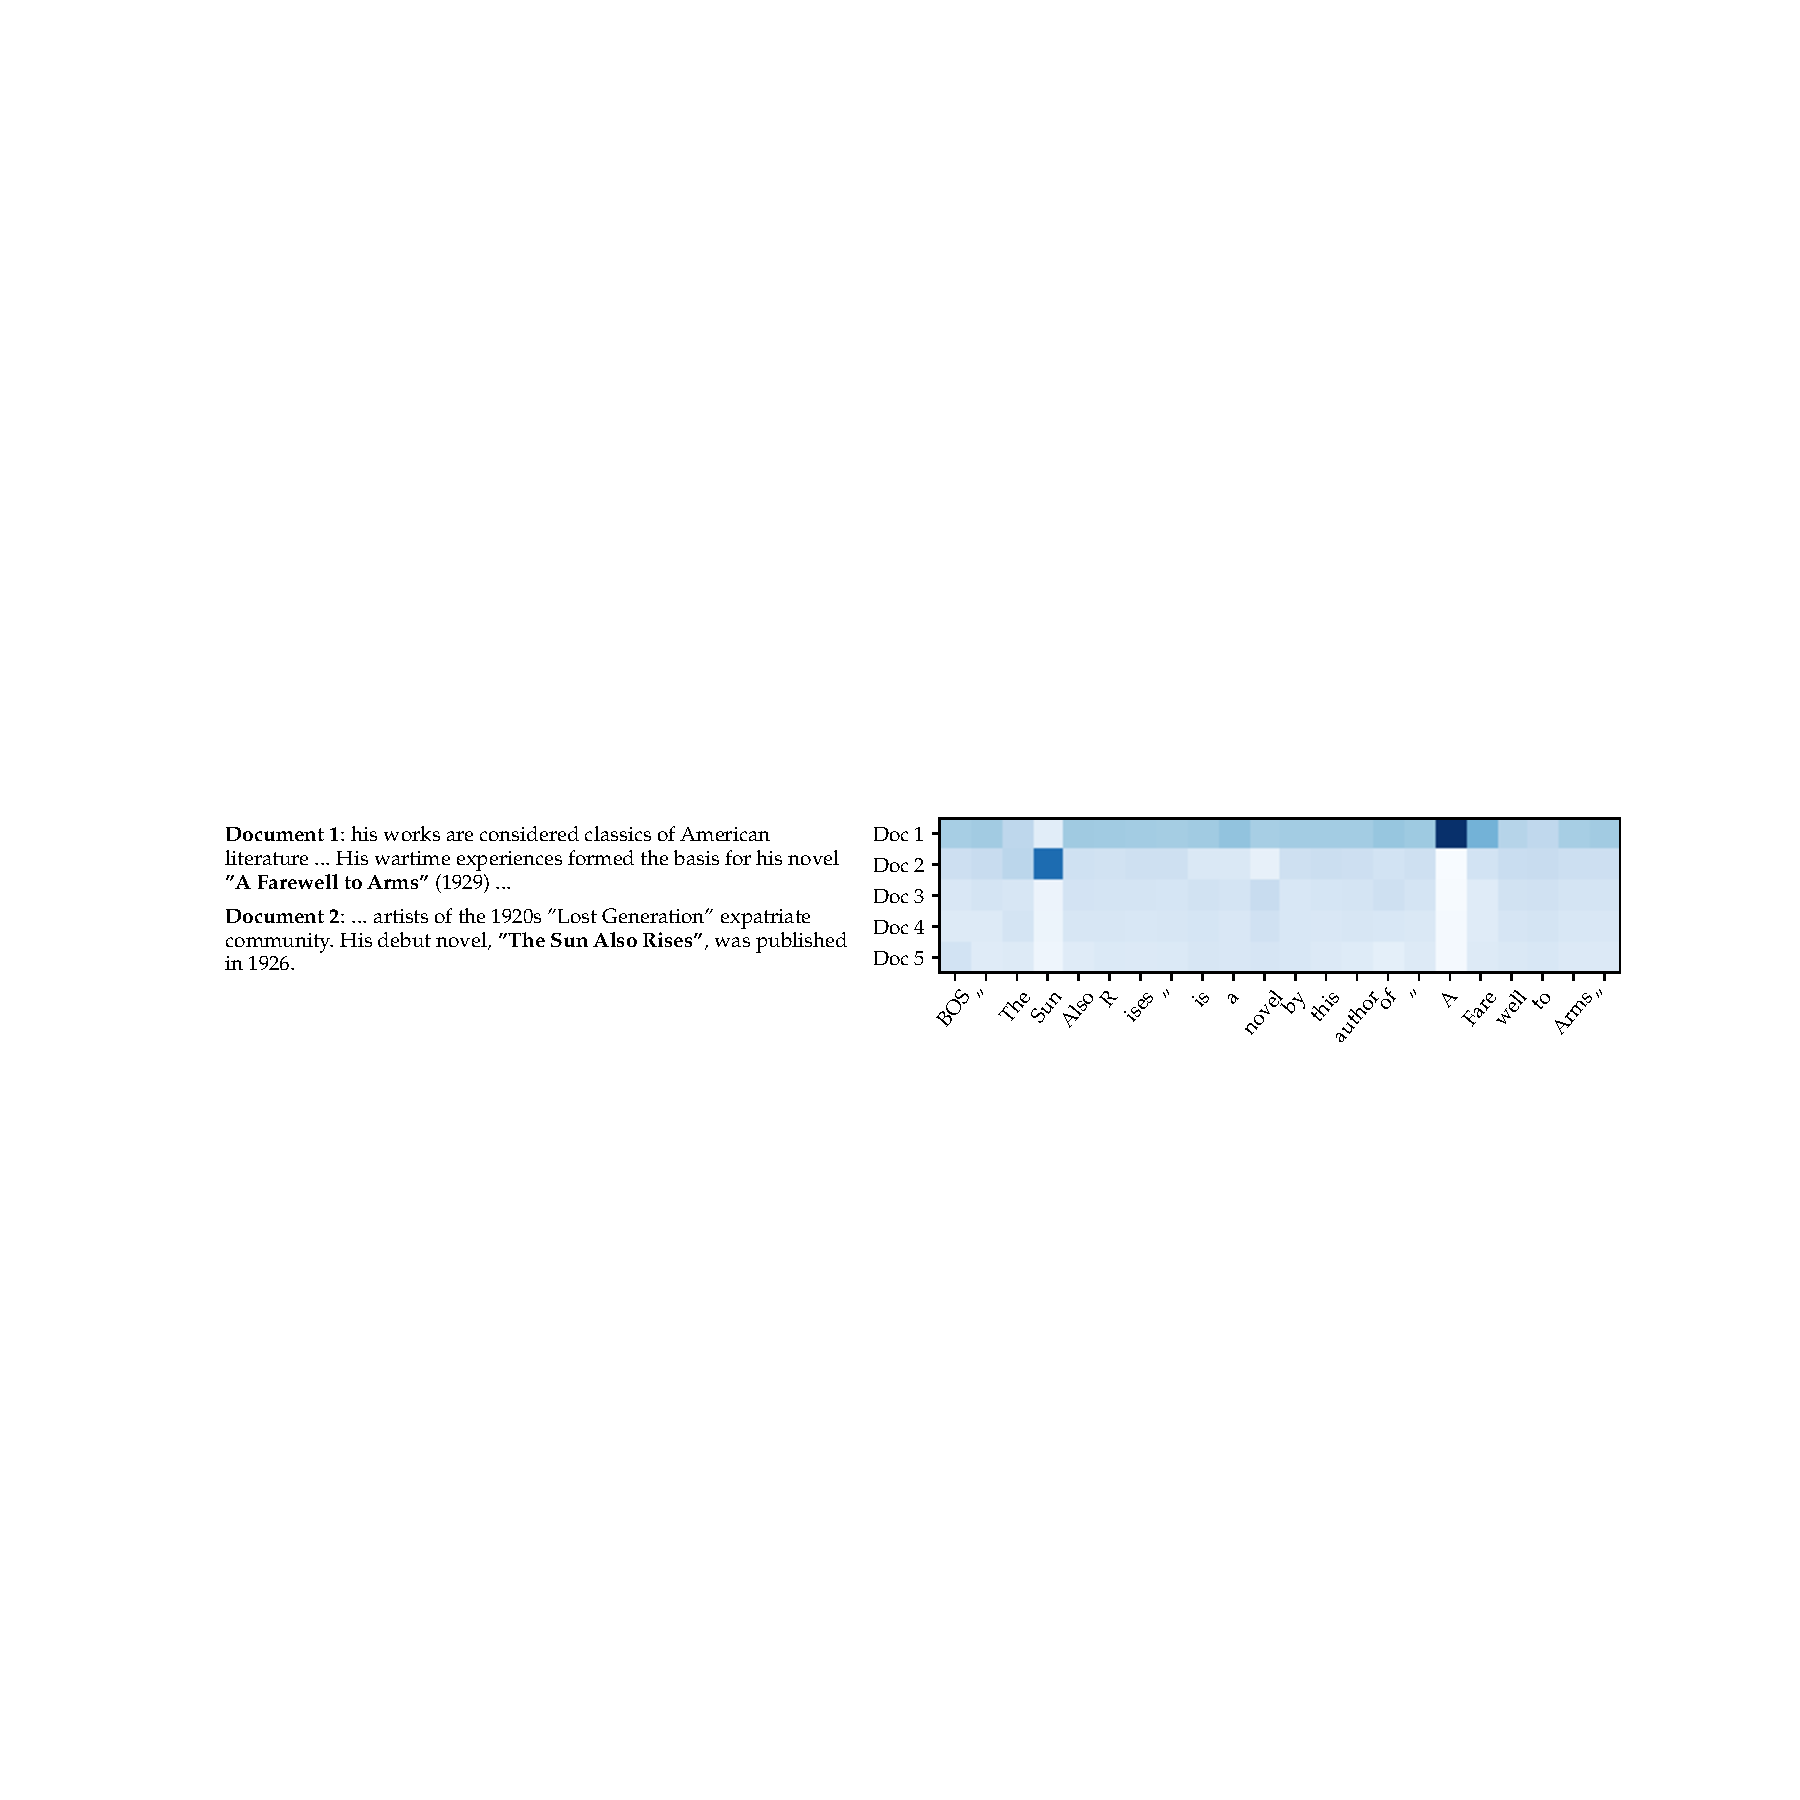
\includegraphics[width=\textwidth]{images/posterior_plot}
  \vspace{-15pt}
\caption{\ragtoken{} document posterior $p(\doc_i|\query, y_i, y_{-i})$ for each generated token for input ``Hemingway" for Jeopardy generation with 5 retrieved documents. The posterior for document 1 is high when generating ``A Farewell to Arms" and for document 2 when generating ``The Sun Also Rises". }
  \label{fig:posterior_plot}
\end{figure*}

\begin{table}[t]
    \centering
    
    \centering %\small 
\small
\setlength{\tabcolsep}{0.3em}
    \caption{Examples from generation tasks. RAG models generate more specific and factually accurate responses. `?' indicates factually incorrect responses, * indicates partially correct responses.}
    \vspace{5pt}
    \resizebox{.99\textwidth}{!}{
    \begin{tabular}{llll}
    \toprule
    Task & Input & Model & Generation  \\
    \midrule
    \multirow{6}{1.2cm}{MS-MARCO} & \multirow{3}{1.8cm}{define middle ear} & BART  & \textsuperscript{?}\footnotesize{The middle ear is the part of the ear between the middle ear and the nose.} \\
    & & RAG-T  & \footnotesize{The middle ear is the portion of the ear internal to the eardrum.} \\
    & & RAG-S & \footnotesize{The middle ear includes the tympanic cavity and the three ossicles.} \\
    \cmidrule{2-4}
     & \multirow{3}{1.8cm}{what currency needed in scotland} & BART  & \footnotesize{The currency needed in Scotland is Pound sterling.} \\
    & & RAG-T  &  \footnotesize{Pound is the currency needed in Scotland.}
 \\
    & & RAG-S  & \footnotesize{The currency needed in Scotland is the pound sterling.}
  \\
    \midrule
    \multirow{6}{1.2cm}{Jeopardy Question Gener -ation} & \multirow{3}{1.8cm}{Washington} & BART  & \textsuperscript{?}\footnotesize{This state has the largest number of counties in the U.S.} \\
    & & RAG-T  & \footnotesize{It's the only U.S. state named for a U.S. president} \\
    & & RAG-S  & \footnotesize{It's the state where you'll find Mount Rainier National Park} \\    \cmidrule{2-4}

     & \multirow{3}{1.8cm}{The Divine Comedy
} & BART  & \textsuperscript{*}\footnotesize{This epic poem by Dante is divided into 3 parts: the Inferno, the Purgatorio \& the Purgatorio}\\
    & & RAG-T  & \footnotesize{Dante's "Inferno" is the first part of this epic poem}\\
    & & RAG-S  & \footnotesize{This 14th century work is divided into 3 sections: "Inferno", "Purgatorio" \& "Paradiso"}\\

    \bottomrule
    \end{tabular}
    }
    \label{tab:examples}
\end{table}



\begin{table}[t]
\begin{minipage}[b]{0.49\linewidth}
\centering
\small
\caption{Human assessments for the Jeopardy Question Generation Task.}
\vspace{5pt}
    \begin{tabular}{lcc}
    \toprule
    &  Factuality & Specificity \\
    \midrule
    BART better & 7.1\% & 16.8\%\\
    RAG better & \textbf{42.7\%} & \textbf{37.4\%} \\
    Both good & 11.7\% & 11.8\%\\
    Both poor & 17.7\% & 6.9\% \\
    No majority & 20.8\% & 20.1\% \\
    \bottomrule
    \end{tabular}
    
    \label{tab:jeopardy}
\end{minipage}
\hspace{0.01\linewidth}
\begin{minipage}[b]{0.49\linewidth}
\centering
 \small
\caption{Ratio of distinct to total tri-grams  for generation tasks.}
\vspace{10pt}
    \begin{tabular}{lcc}
    \toprule
    &   \multicolumn{1}{m{2cm}}{\centering MSMARCO} &  \multicolumn{1}{m{2cm}}{\centering Jeopardy QGen} \\
    \midrule
    Gold  & 89.6\% & 90.0\%\\
    BART  & 70.7\% & 32.4\%\\
    RAG-Token & 77.8\% & 46.8\%\\
    RAG-Seq. & 83.5\% & 53.8\%\\
    \bottomrule
    \end{tabular}

    \label{tab:diversity}
\end{minipage}
\end{table}


\subsection{Fact Verification}

Table \ref{tab:generations} shows our results on FEVER. For 3-way classification, RAG scores are within 4.3\% of state-of-the-art models, which are complex pipeline systems with domain-specific architectures and substantial engineering, trained using intermediate retrieval supervision, which RAG does not require. For 2-way classification, we compare against \citet{Thorne2020AvoidingCF}, who train RoBERTa~\cite{liu-etal-2019-robust} to classify the claim as true or false given the gold evidence sentence. RAG achieves an accuracy within 2.7\% of this model, despite being supplied with only the claim and retrieving its own evidence.
We also analyze whether documents retrieved by RAG correspond to documents annotated as gold evidence in FEVER. 
We calculate the overlap in article titles between the top $k$ documents retrieved by RAG and gold evidence annotations.
We find that the top retrieved document is from a gold article in 71\% of cases, and a gold article is present in the top 10 retrieved articles in 90\% of cases.

\subsection{Additional Results}
\label{sec:gen_div}

\paragraph{Generation Diversity} Section \ref{sec:fact_generation_results} shows that RAG models are more factual and specific than BART for Jeopardy question generation. Following recent work on diversity-promoting decoding  \cite{li-etal-2016-diversity,Vijayakumar2016DiverseBS,massarelli2019decoding}, we also investigate generation diversity by calculating the ratio of distinct ngrams to total ngrams generated by different models. Table \ref{tab:diversity} shows that \raganswer{}'s generations are more diverse than \ragtoken{}'s, and both are significantly more diverse than BART
without needing any diversity-promoting decoding.
\begin{table}[t]

    \centering
    \small
        \caption{Ablations on the dev set. As FEVER is a classification task, both RAG models are equivalent.}
        \vspace{5pt}
    \begin{tabular}{lllll|llll|cc}
    \toprule
         \multicolumn{1}{c}{Model} & \multicolumn{1}{c}{NQ} & \multicolumn{1}{c}{TQA} & \multicolumn{1}{c}{WQ} & \multicolumn{1}{c}{CT} & \multicolumn{2}{c}{Jeopardy-QGen} & \multicolumn{2}{c}{MSMarco} & \multicolumn{1}{c}{FVR-3} & \multicolumn{1}{c}{FVR-2} \\
         \multicolumn{1}{c}{} & \multicolumn{4}{c}{Exact Match} &   \multicolumn{1}{c}{B-1} & \multicolumn{1}{c}{QB-1} &\multicolumn{1}{c}{R-L} & \multicolumn{1}{c}{B-1} & \multicolumn{2}{c}{Label Accuracy} \\
         \midrule
        \ragtoken{}-BM25 & 29.7&	41.5&	32.1&	33.1 & 17.5 &	22.3&	55.5 &	48.4 & \textbf{\multirow{ 2}{*}{75.1}} & \textbf{\multirow{ 2}{*}{91.6}}\\
        RAG-Sequence-BM25 & 31.8&	44.1&	36.6&	33.8 & 11.1	& 19.5	&56.5 &	46.9 \\
        \midrule
        \ragtoken{}-Frozen & 37.8 &	50.1 &	37.1&	51.1 & 16.7	&21.7&	55.9 &	49.4 & \multirow{ 2}{*}{72.9} & \multirow{ 2}{*}{89.4} \\
        RAG-Sequence-Frozen & 41.2	& 52.1&	41.8&	52.6 & 11.8	& 19.6&	56.7 &	47.3 \\
        \midrule
        \ragtoken{} & 43.5&	54.8&	\textbf{46.5}&	51.9 & \textbf{17.9}	& \textbf{22.6} &	56.2&	\textbf{49.4}& \multirow{ 2}{*}{74.5} & \multirow{2}{*}{90.6}\\
        RAG-Sequence & \textbf{44.0}&	\textbf{55.8}&	44.9 &	\textbf{53.4} & 15.3&	21.5 &	\textbf{57.2} &	47.5\\
    \bottomrule
    \end{tabular}

    \label{tab:ablations}
\end{table}
\paragraph{Retrieval Ablations} A key feature of RAG is learning to retrieve relevant information for the task.
To assess the effectiveness of the retrieval mechanism, we run ablations where we freeze the retriever during training.
As shown in Table \ref{tab:ablations}, learned retrieval improves results for all tasks.

We compare RAG's dense retriever to a word overlap-based BM25 retriever~\cite{robertson2009bm25}. Here, we replace RAG's retriever with a fixed BM25 system, and use BM25 retrieval scores as logits when calculating $p(\doc|\query)$. Table \ref{tab:ablations}
shows the results.
For FEVER, BM25 performs best, perhaps since FEVER claims are heavily entity-centric and thus well-suited for word overlap-based retrieval.
Differentiable retrieval improves results on all other tasks, especially for Open-Domain QA, where it is crucial.


\paragraph{Index hot-swapping}An advantage of non-parametric memory models like RAG is that knowledge can be easily updated at test time. Parametric-only models like T5 or BART need further training to update their behavior as the world changes. To demonstrate, we build an index using the DrQA~\cite{chen_reading_2017} Wikipedia dump from December 
2016 and compare outputs from RAG using this index to the newer index from our main results (December 
2018). We prepare a list of 82 world leaders who had changed between these dates and use a template ``Who is \{position\}?'' (e.g. ``Who is the President of Peru?'') to query our NQ RAG model with each index.
RAG answers 70\% correctly using the 2016 index for 2016 world leaders and 68\% using the 2018 index for  2018 world leaders. 
Accuracy with mismatched indices is low 
(12\% with the 2018 index and 2016 leaders, 4\% with the 2016 index and 2018 leaders). 
This shows we can update RAG's world knowledge by simply replacing its 
non-parametric memory.

\paragraph{Effect of Retrieving more documents} 
Models are trained with either 5 or 10 retrieved latent documents, and we do not observe significant differences in performance between them. 
We have the flexibility to adjust the number of retrieved documents at test time, 
which can affect performance and runtime.
Figure \ref{fig:n_docs_figures} (left) shows that retrieving more documents at test time monotonically improves Open-domain QA results for \raganswer{}, but performance peaks for \ragtoken{} at 10 retrieved documents. Figure \ref{fig:n_docs_figures} (right) shows that retrieving more documents leads to higher Rouge-L for \ragtoken{} at the expense of Bleu-1, but the effect is less pronounced for \raganswer{}. 

\begin{figure}[h]
\centering

  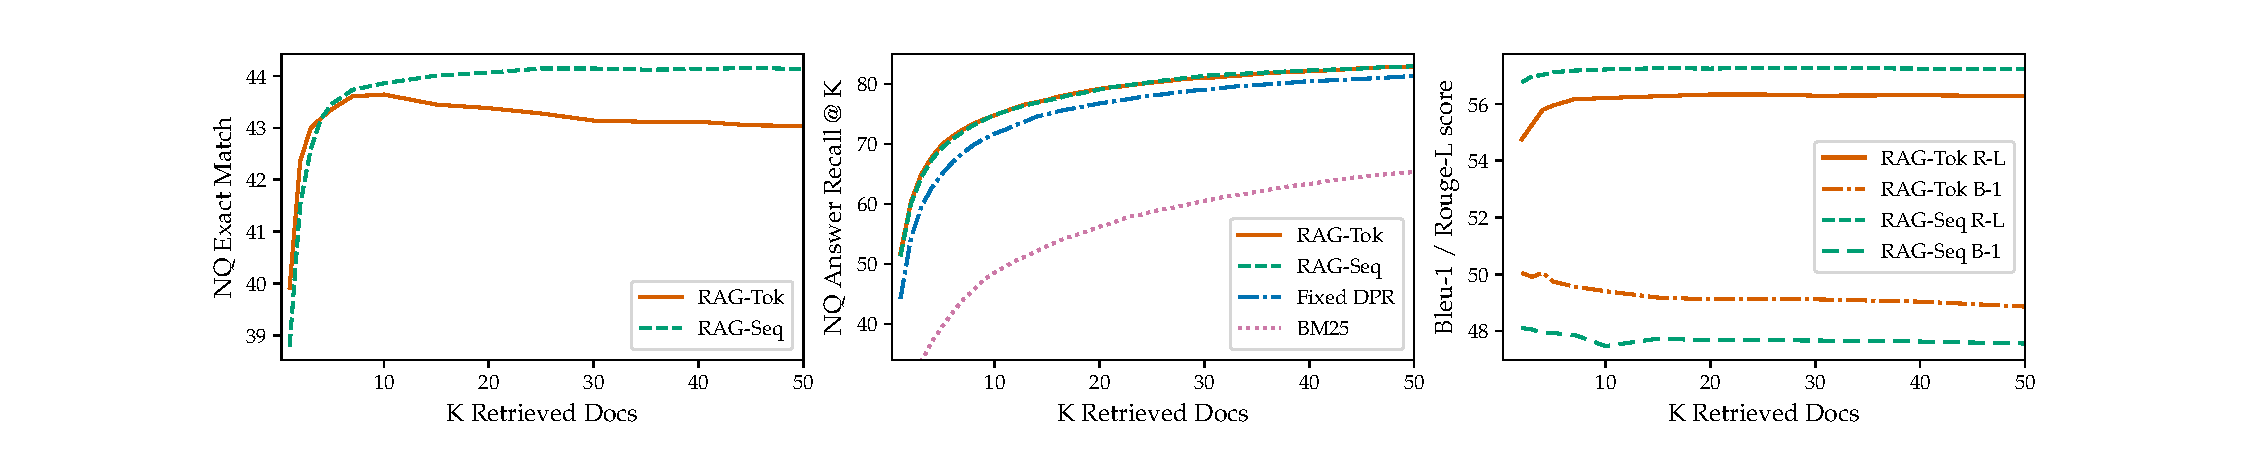
\includegraphics[width=\textwidth]{images/retrieval_plots_flat.pdf}
  \vspace{-17pt}
\caption{Left: NQ performance as more documents are retrieved. Center: 
Retrieval recall performance in NQ.
Right: MS-MARCO Bleu-1 and Rouge-L as more documents are retrieved. 
    }
  \label{fig:n_docs_figures}
\end{figure}